\section{Slagterieksempel}

På Danish Crown slagteriet i Horsens udskæres grisene af en robot.

\begin{quote}\textit{``Grisen [\ldots] skal nu skæres i mindre, håndterbare stykker. Det sker i en meget avanceret maskine -- en såkaldt tredeler -- hvor hver halvdel af grisen deles i tre stykker: bov, mellemstykke og skinke. \\ 
\\
Robotten starter med at fotografere hver halvdel. Dataene fra billedet kombineres med ordren og kundens ønsker, hvorefter stykket deles i tre - nøjagtigt afpasset kundens ønsker.''}{ Danish Crowns hjemmeside\footnote{http://www.danishcrown.dk/custom/horsens/3772.asp}}\end{quote}

Et billede af den automatiske tredeler er vist  på \cref{fig:pig}. Vi forestiller os at selve udskæring også laves på baggrund af en model af hvordan grisen er udformet. Det har dog vist sig at modellen ikke altid resulterer i en  optimal udskæring, da  ca. 10\% af alle grise har et ekstra sæt ribben, som modellen ikke tager højde for. Til at løse dette problem har slagteriet udviklet en ny model for grise med et ekstra sæt ribben.

\begin{figure}
 \begin{center}
  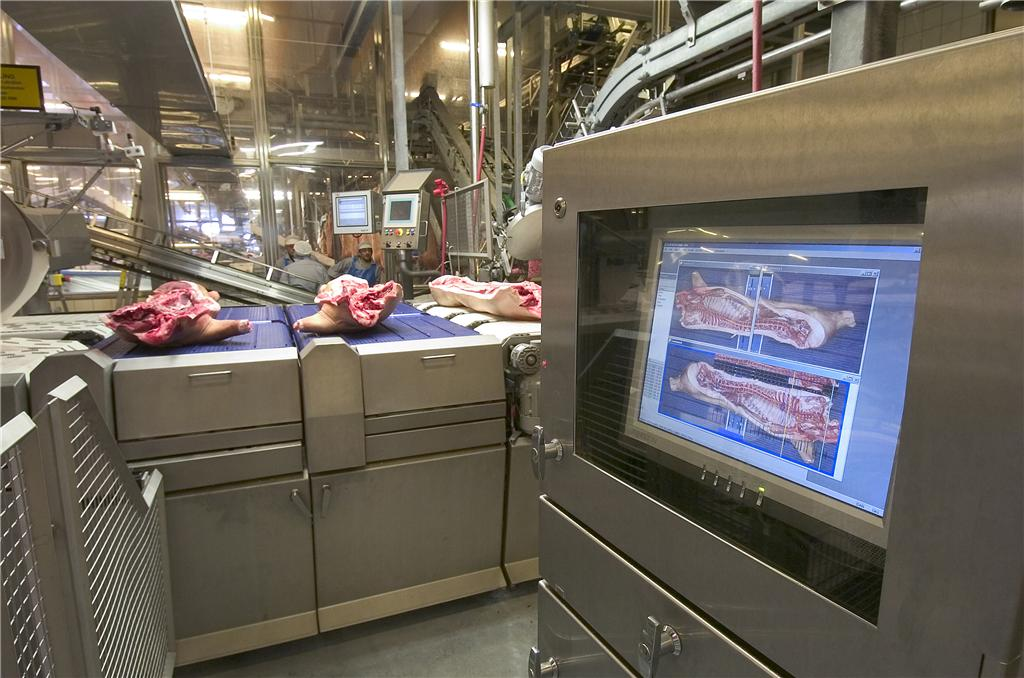
\includegraphics[scale=0.5]{images/209690-1}
	\caption{Billedet viser i forgrunden  et foto taget af tredeleren til brug for analyse. I baggrunden ses transportbåndet, hvor de halve  grise venter på på at blive udskåret af den automatisk tredeler.}
	\label{fig:pig}
\end{center}
\end{figure}

I det første eksempel på en applikation der kan bruge et RTP systemer, skal vi udvikle er en beslutningsmodel, der kan beslutte hvilken model robotten skal bruge til at  udskære den enkelte gris med. 

Slagteriet har placeret kameraet i starten af et transportbåndet mens udskæringsrobotten findes i den anden enden. Der kan være flere svin på transportbåndet på samme tid, og det fremføre svinene i et fast tempo. Dette giver et fast tidsrum fra svinet passere kameraet til det passere robotten. Vi har hermed et klassisk RTP system, hvor robotten skal foretage et valg af model under en hard deadline, da det ikke er en mulighed ikke at foretage en udskæring.

Vi må først se på arbejdsgangen der er involveret i valget af model. 
\begin{enumerate}
\tightlist
	\item Et billede bliver taget af svinet mens den passere kameraet.
	\item Billedet konverteres til en 3D-model af svinet.
	\item 3D-modellen analyseres.
	\item Modellen udvælges på baggrund af analysen, ordren og kundens ønske.
	\item Robotten udskærer grisen.
\end{enumerate}

Man kan se at arbejdsgangen indeholder en  række klart afgrænsede arbejdsområder, som med fordel kan modelleres som selvstændige processer i \pycsp. Der findes do ikke kun en måde at opbygge procesnetværket på, men vi har valgt at have følgende processer: Røntgenskanner, Billedekonvertering, 3D-analyse og en udvælgelse og udskæringsproces, hvilket leder til et procesnetværk som vist i \cref{fig:pig-network}.

\begin{figure}
 \begin{center}
  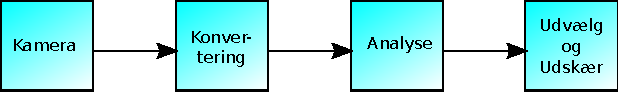
\includegraphics[scale=1]{images/pig-network}
	\caption{Procesnetværk til udskæring af svin på et slagteri.}
	\label{fig:pig-network}
\end{center}
\end{figure}

Den simple model, viser dog ikke den store fordel, ved RTP systemet i \pycsp, som er at netværket nemt kan udvide antallet af processer til at passe det endelige opstilling. Som programmør har man mulighed for at teste forskellige indstillinger i netværket, som hvor mange processer der samtidigt skal konverterer billederne og hvor mange analyser skal kunne foregå samtidigt. Endeligt kan systemet også nemt udvides hvis det overordnede design på slagteriet ændre sig. Viser det sig f.eks at røntgenskanneren holder netværket tilbage kan man blot udvide procesnetværket med endnu en røngtenproces.

\subsubsection*{Implementering i Greenletsversionen}
Til at implementere eksemplet uden brug af af RTP-udvidelsen i \pycsp, kan vi oprette hvert svin som et objekt og tilknytte en deadline. Nu kan hver proces evaluere om svinet har overskredet sin deadline, i det tilfælde fjerne svinet, og stoppe den videre behandling. Det er ikke angivet hvordan hele processen startes, men vi antager der findes en form for detektor foran røngtenkameraet, der opfanger når et svin passere og som dermed  starter processen. 
Når detektoren starter hele processen, opretter den svineobjektet som den sender til Røngtenprocessen, samt sender en kopi direkte til udvælgelse og udskæringsprocessen. dermed ved processen at der ankommer et svin som den skal udskære, og hvis den inden deadline får en analyse af svinet, kan den træffe et begrundet valg om hvilken model der skal bruges,  men hvis ikke denne analyse findes, bruges blot standardmodellen. \CRef{fig:pig-network2} viser det endelige  netværk, hvor detektoren er introduceret, og som sender data til hhv. Røntgenprocessen og til Udvælgelse og udskæringsprocessen. 

\begin{figure}
 \begin{center}
  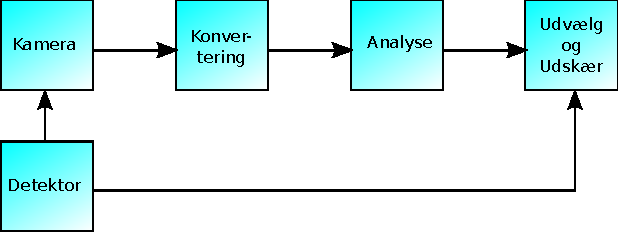
\includegraphics[scale=1]{images/pig-network2}
	\caption{Procesnetværk med detektor til initiering af hvert svin.}
	\label{fig:pig-network2}
\end{center}
\end{figure}

Et problem ved at implementere hele slagterieksemplet i \pycsp er  grænsefladen mellem verden hvor svinene kører på transportbåndet, og den elektroniske verden, der bygger på greenletsversionen, og hvor  kun en proces kan være aktiv af gangen. For hele tiden at arbejde kører konvertering og analyse processen, mens  udskæringsprocessen venter på at svinene kommer inden for rækkevidde. Men konvertering og analysen processen  skal frivilligt afgive kontrollen, mens svinet er indenfor robottens rækkevidden og hvis de ikke gør, bliver svinet ikke udskåret. Dette er dybt uhensigstmæssigt 



%\subsection{Eksempel 2 - Sensornetværk med høj/lav -prioritet}
%\inline{eks2: skal vise alternation, kan være en sensor som modtager måledata med lav prioritet og som skal sende måledata på opdordring med høj prioritet.}
